\documentclass[ignorenonframetext]{beamer} 
\usepackage[utf8]{inputenc} 
\usepackage{amsmath} 
\usepackage{amsfonts} 
\usepackage{amssymb} 
\usepackage[font=small]{caption} 

\renewcommand{\figurename}{Abb.} 

\mode<presentation> 
{ 
  \usetheme{Singapore} 
  \usecolortheme[named=darkgray]{structure} 

} 

%Standard Angaben
%\author{ }
%\title{ }
%\date{ }
\begin{document}
%---------------------------------------------1 FOLIE ---------------------------------------------
\hfill%
\begin{frame} 
\frametitle{Flashtalk 19.10.15 - Dessert Ant Adaptive Navigation} 
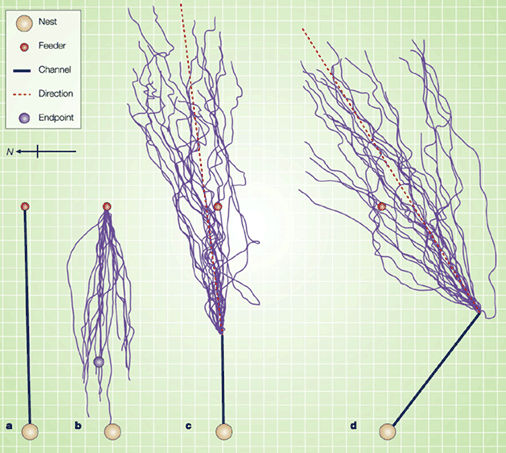
\includegraphics[scale=0.2]{nature.png}\\
\footnote{Nature ,542-552 (July 2002)  }

\begin{itemize}
	\item Pathfinder: Pathintegration, pheromones, visual landmarks 
	\begin{itemize}
%	\item how are these three pathinding modes combined ?
	\item do the simulated pattern match the empirical ones ?
	\item how does the memory affect the path pattern ?
%	\item Can the ants survive if the landmarks constantly change?
	\item ...
	\end{itemize}
\item The Model:
	\begin{itemize}
	\item Agent-Based Model with individual ants as agents
	\item various variables have to be traced such as
		\begin{itemize}
		\item nestLocation, foodLacation, phermoneparticles, ants, landmarks
		\end{itemize}
	
	\end{itemize}
\end{itemize}
\end{frame} 
\end{document}